% Split from part3.tex: ITES section
\chapter{Развитие иерархического безопасного обучения с подкреплением с использованием модели мира}
\label{ch:ites}

В предыдущей главе был рассмотрен метод SG-Safe, использующий генерацию промежуточных подцелей для улучшения исследовательских способностей безопасной стратегии. Однако в SG-Safe безопасность самих подцелей не гарантируется явно: подцели используются как обучающий сигнал, но их безопасность возникает эмпирически через согласование с распределением посещаемых состояний. Метод ITES, рассматриваемый в данной главе, решает более сильную задачу: обеспечить безопасность как при выборе промежуточных подцелей, так и при их достижении низкоуровневой стратегией (рис.~\ref{fig:ites_conceptual_scheme}).

Основная проблема состоит в том, что существующие методы безопасного обучения с подкреплением плохо работают в задачах с большим горизонтом. Одноуровневые безопасные стратегии часто не способны одновременно исследовать среду, достигать удалённой цели и соблюдать ограничения безопасности: они либо нарушают ограничения, либо становятся чрезмерно консервативными и не находят успешное поведение. Эта проблема особенно выражена в задачах с длинной последовательностью действий, сложной динамикой агента, высокой размерностью пространства действий или разреженным вознаграждением.

Метод ITES~\cite{gorbov2026ites} (Imagine To Ensure Safety in Hierarchical Reinforcement Learning) продолжает линию иерархического безопасного обучения, но делает отдельный акцент на безопасности самой иерархии. В SG-Safe подцели в основном помогали безопасной стратегии лучше исследовать среду. В ITES дополнительно проверяется, какие подцели предлагает верхний уровень и насколько безопасно низкоуровневая стратегия движется к выбранной подцели.

\begin{figure}[t]
    \centering
    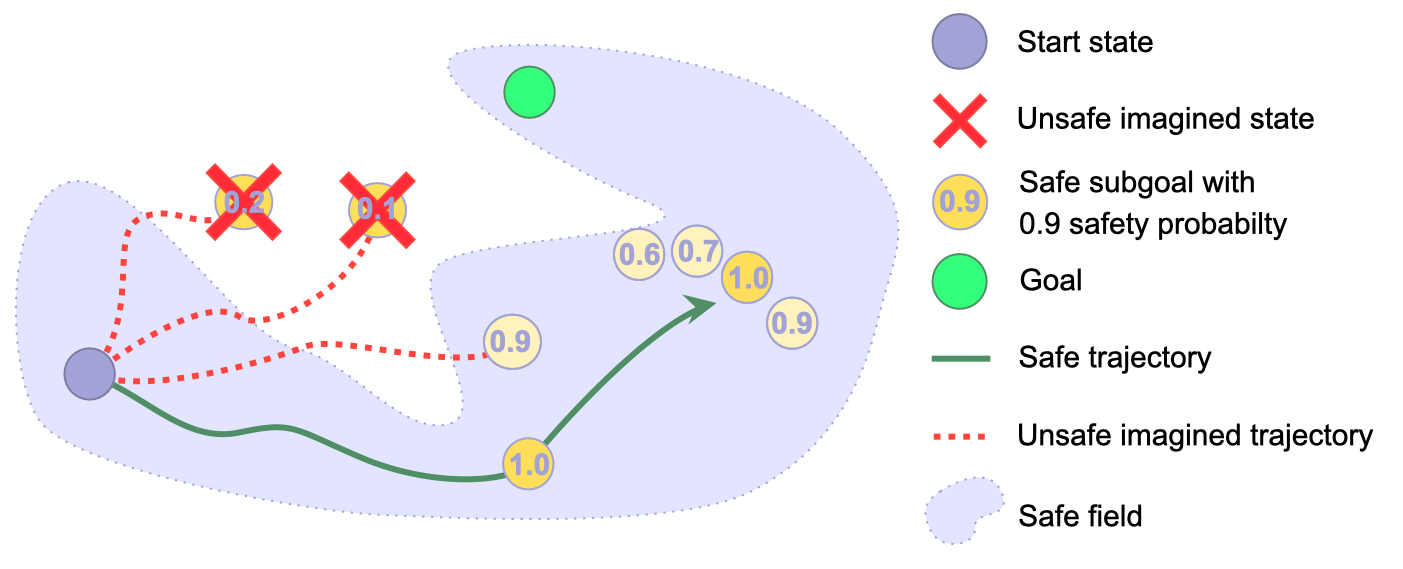
\includegraphics[width=0.85\textwidth]{conceptual_scheme.png}
    \caption{Схема метода ITES. Верхний уровень выбирает промежуточные подцели с учётом штрафов, а нижний уровень проверяет безопасность движения к ним с помощью модели мира.}
    \label{fig:ites_conceptual_scheme}
\end{figure}

\section{Метод ITES}
\label{sec:ites_method}

Предложенный подход обеспечивает безопасность на двух взаимодополняющих уровнях: при генерации безопасных подцелей и при безопасном достижении выбранных подцелей. Для генерации подцелей, расположенных в безопасной области пространства состояний, используется модель штрафов $C_M$, классифицирующая состояния как безопасные или небезопасные, а также верхнеуровневый критик штрафов $Q^h_c(s, s_g, g)$, оценивающий ожидаемые накопленные штрафы при выборе подцели $s_g$. Эти компоненты направляют верхнеуровневую стратегию к подцелям, которые одновременно являются безопасными и достижимыми.

Для безопасного достижения выбранных подцелей используется модель мира $M$, предсказывающая короткие фрагменты траектории в виде переходов $s' = M_{\theta_m}(s, a)$. В сочетании с моделью штрафов $C_M$ модель мира позволяет оценивать безопасность низкоуровневых траекторий до выполнения действий в среде. Благодаря этому низкоуровневая стратегия может избегать небезопасного поведения при движении к заданной подцели.

\noindent\textbf{Иерархическая структура.}
В качестве базового алгоритма используется HRAC~\cite{hrac} (Hierarchical Reinforcement Learning with $k$-step Adjacency Constraint). Данный метод включает две стратегии: верхнеуровневую стратегию $\pi^h_{\theta_h}(s_g|s, g)$ и низкоуровневую стратегию $\pi^l_{\theta_l}(a|s, s_g)$. Основная идея HRAC состоит в генерации подцелей, расположенных на заданном расстоянии $k$ от текущего состояния агента. Для этого используется сеть смежности $\psi$, которая отображает каждое состояние $s$ в его векторное представление $\psi(s)$. Данная сеть обучается с использованием следующей функции потерь:
\begin{equation}
    \label{eq:hrac_adj_loss}
    \begin{split}
    L_{adj}
    &= \mathbb{E}_{s_i,s_j \in \mathcal{S}}
    \Bigl[
        l \cdot
        \max\left(
            \|\psi(s_i)-\psi(s_j)\| - \epsilon, 0
        \right)
        + \\
    &\quad (1-l)\cdot
        \max\left(
            \epsilon+\delta-\|\psi(s_i)-\psi(s_j)\|,0
        \right)
    \Bigr].
    \end{split}
\end{equation}
где $\delta > 0$ задаёт зазор между векторными представлениями, $\epsilon$ является масштабирующим коэффициентом, а $l\in\{0, 1\}$ обозначает метку $k$-шаговой смежности. Эта функция потерь позволяет обучить сеть смежности так, чтобы для состояний $s_i$ и $s_j$, достижимых друг из друга за $k$ шагов, выполнялось условие $\|\psi(s_i) - \psi(s_j)\| < \epsilon$.

Далее сеть смежности используется при обновлении верхнеуровневой стратегии на основе алгоритма TD3~\cite{td3}. Для этого в функцию потерь верхнеуровневой стратегии добавляется дополнительный член:
\begin{equation}
    \label{eq:hrac_high_level_loss}
    L^h
    =
    -Q^h_{\theta_{qh}}(s, s_g, g)
    +
    \beta^h_{adj} L_{adj}(s, s_g),
\end{equation}
где $\beta^h_{adj}$ — коэффициент при функции потерь смежности, являющийся масштабирующим гиперпараметром. Для низкоуровневой стратегии используется алгоритм TD3 без дополнительных модификаций со следующей функцией потерь:
\begin{equation}
    \label{eq:hrac_low_level_loss}
    L^l
    =
    -Q^l_{\theta_{ql}}(s, a, s_g),
\end{equation}
где $Q^h_{\theta_{qh}}$ и $Q^l_{\theta_{ql}}$ --- два критика вознаграждений верхнего и низкого уровня соответственно, аппроксимируемые нейронными сетями и оценивающие дисконтированную внешнюю и внутреннюю награды соответственно.

HRAC позволяет решать задачи с большим горизонтом, однако не может быть напрямую применён в постановке марковского процесса принятия решений с ограничениями. Далее показывается, как обеспечить безопасность как при генерации подцелей, так и при исполнении низкоуровневой стратегии.

\subsection{Безопасность на верхнем уровне: генерация безопасных подцелей}
\label{subsec:ites_safe_subgoal_generation}

Схема обновления верхнеуровневой стратегии приведена на рис.~\ref{fig:ites_learning_scheme}. Обновление выполняется на основе переходов $\langle s, s_g, R^h \rangle$ и таких модулей, как модель штрафов $C_M$ и критика вознаграждений $Q^h_{\theta_{qh}}$, которые оценивают безопасность и полезность сгенерированной подцели.

\begin{figure}[t]
    \centering
    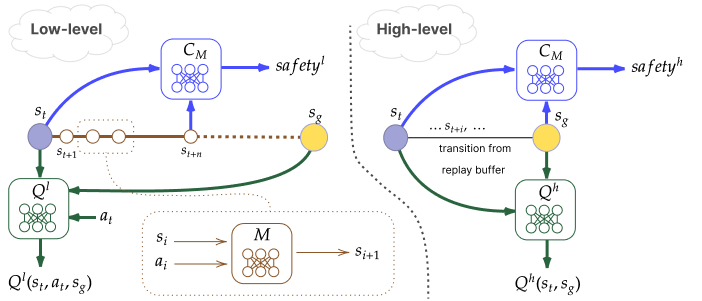
\includegraphics[width=0.9\linewidth]{learning_scheme_1.png}
    \caption{Схема обучения низкоуровневой и верхнеуровневой стратегий. \textbf{Слева}: модель штрафов $C_{M}$ и модель мира $M$ отвечают за обеспечение безопасности при обновлении низкоуровневой стратегии, тогда как функция $Q^l_{\theta_{ql}}$ используется для оптимизации награды. \textbf{Справа}: модель штрафов $C_{M}$ используется для учёта безопасности при обновлении верхнеуровневой стратегии, а функция $Q^h_{\theta_{qh}}$ используется для оптимизации награды.}
    \label{fig:ites_learning_scheme}
\end{figure}

\textbf{Модель штрафов.} Задача модели штрафов $C_M$ состоит в предсказании вероятности того, что произвольная подцель $s_g$ является безопасной, с использованием локальной информации о состоянии $s$:
\begin{equation}
    \label{eq:ites_high_level_safety}
    safety^h(s_g,s)
    =
    C_M(s_g,s)
    \in [0,1].
\end{equation}

Поскольку в экспериментах функция штрафов $c$ зависит только от состояния, $c:\mathcal{S}\rightarrow[0,1]$, модель штрафов может использоваться для предсказания значения штрафов состояний. Однако в данной работе предлагается рассматривать безопасность подцелей как вероятность их безопасности. Оптимизация такой величины способствует генерации подцелей, находящихся дальше от границы между безопасными и небезопасными состояниями. Для реализации модели штрафов используется нейронная сеть, а именно многослойный перцептрон, параметризованный $\theta_c$. В качестве функции потерь для обучения используется бинарная кросс-энтропия. Модель обучается в онлайн-режиме с использованием того же буфера опыта, который используется для модели мира $M$.

Модель штрафов использует только локальные наблюдения о препятствиях, однако остаётся достаточно точной для предсказания безопасности ближайших подцелей, поскольку HRAC генерирует подцели на коротком горизонте $s_g$ в пределах наблюдаемой области.

\textbf{Целевая функция верхнеуровневой стратегии.} Чтобы верхнеуровневая стратегия генерировала безопасные подцели, в функцию потерь HRAC (формула~\ref{eq:hrac_high_level_loss}) был добавлен член $L_{safety^h}(s, s_g)=-safety^h(s_g, s)$ с коэффициентом $\beta^h_{safe}$, отвечающим за вклад безопасности:
\begin{equation}
    \label{eq:ites_high_level_safety_loss}
    L_{safety^h}(s,s_g)
    =
    -safety^h(s_g,s).
\end{equation}

Итоговая функция потерь высокоуровневой стратегии записывается как:
\begin{equation}
    \label{eq:ites_safe_manager}
    L^h
    =
    -Q^h_{\theta_{qh}}(s,s_g,g)
    +
    \beta^h_{adj} L_{adj}(s,s_g)
    +
    \beta^h_{safe} L_{safety^h}(s,s_g),
\end{equation}
где $\beta^h_{safe}$ задаёт вес компоненты безопасности.

\noindent
Эксперименты показали, что использования только модели штрафов $C_M$ для генерации безопасных подцелей недостаточно. В этом случае верхнеуровневая стратегия может научиться предсказывать подцели, находящиеся в безопасных областях, но недостижимые для низкоуровневой стратегии. Например, подцель может быть расположена за препятствием, что вынуждает низкоуровневую стратегию решать задачу обхода препятствий с большим горизонтом. Для решения этой проблемы используется верхнеуровневый критик штрафов $Q^h_c(s, s_g, g)$, который оценивает ожидаемую дисконтированные штрафы до конца эпизода. Он добавляется в целевую функцию верхнеуровневой стратегии, а множитель Лагранжа $\lambda$ обучается адаптивно для выполнения ограничения безопасности $Q^h_c(s, s_g, g) \leq d$. Итоговая целевая функция верхнеуровневой стратегии имеет вид:
\begin{equation}
    \label{eq:ites_high_level_policy_update}
    L^h
    =
    -Q^h_{\theta_{qh}}(s,s_g,g)
    +
    \beta^h_{adj} L_{adj}(s,s_g)
    +
    \beta^h_{safe} L_{safety^h}(s,s_g)
    +
    \lambda Q^h_c(s,s_g,g).
\end{equation}

Множитель Лагранжа $\lambda$ обновляется с помощью градиентного спуска и проецируется на область $\lambda \ge 0$:
\begin{equation}
    \label{eq:ites_lambda_update}
    \lambda
    \leftarrow
    \left[
        \lambda
        +
        \left(
            Q^h_c(s,s_g,g)-d
        \right)
    \right]_+.
\end{equation}

Верхнеуровневый критик штрафов $Q^h_c(s, s_g, g)$ обучается стандартной беллмановской регрессией на верхнеуровневых переходах, аналогично критику награды, с использованием накопленных штрафов, собранной за соответствующий $k$-шаговый интервал достижения подцели.

\subsection{Безопасность на нижнем уровне: безопасное достижение подцелей}
\label{subsec:ites_low_level_safety}

Модель штрафов используется для оценки подцелей, сгенерированных верхнеуровневой стратегией, и для их оптимизации в сторону безопасных подцелей. Однако даже если выбранная подцель является безопасной, агент может нарушить ограничения безопасности в процессе её достижения. Например, мобильный робот может чрезмерно ускориться при движении к подцели. Для решения этой проблемы используется комбинация модели штрафов и модели мира, что соответствует левой части схемы на рис.~\ref{fig:ites_learning_scheme}.

Пусть для агента задана текущая подцель $s_g$. Для проверки безопасности в воображении последовательно генерируются действия с помощью низкоуровневой стратегии $a \sim \pi^l_{\theta_l}(a|s, s_g)$, после чего модель мира используется для получения следующего состояния $s' = M_{\theta_m}(s, a)$. Эта процедура повторяется $n$ раз. Здесь $n$ — число шагов воображения, выбираемое из дискретного равномерного распределения $n \sim U(\{1,\ldots,k-1\})$; соответствующая схема показана в левой части рис.~\ref{fig:ites_learning_scheme}. Итоговая безопасность для низкоуровневой стратегии вычисляется с использованием модели штрафов и модели мира следующим образом:
\begin{equation}
    \label{eq:ites_low_level_safety}
    safety^l(s, s_g)
    =
    C_{M}(\phi(s_n), s)
    \in [0, 1].
\end{equation}

Хотя безопасность оценивается только в одном случайно выбранном воображаемом состоянии, равномерный выбор $n$ делает такую оценку несмещённой оценкой средней безопасности воображаемой траектории. Поэтому оптимизация этой величины улучшает безопасность всей траектории в среднем. Использование накопленных штрафов в воображении вместо случайного выбора $n$ показало меньшую устойчивость обучения и худшие показатели безопасности. Это связано с двумя факторами. Во-первых, вычисление значений штрафов через модель штрафов для всех воображаемых состояний может приводить к взрыву градиентов, особенно при больших горизонтах воображения в 10--20 шагов. Во-вторых, для моделей мира характерно накопление ошибки предсказания при увеличении горизонта воображения. Использование случайного состояния для оценки безопасности вместо полного воображаемого развёртывания позволяет избежать длинных вычислительных траекторий и одновременно уменьшить влияние накопленной ошибки модели мира. Кроме того, такой подход снижает время обучения.

Полученное значение $safety^l(s, s_g)$ используется в итоговой функции потерь актора:
\begin{equation}
    \label{eq:ites_low_level_policy_update}
    \begin{split}
    L^l
    &= -Q^l_{\theta_{ql}}(s, a, s_g)
    + \beta^l_{safe} L_{safety^l}(s, s_g), \\
    L_{safety^l}(s, s_g)
    &= -safety^l(s, s_g).
    \end{split}
\end{equation}

Здесь $\beta^l_{safe}$ — гиперпараметр, аналогичный $\beta^h_{safe}$ из формулы~\ref{eq:ites_safe_manager}. Воображаемая безопасность может быть добавлена как дополнительный член функции потерь верхнеуровневой стратегии, а не низкоуровневой. Однако генерация подцелей является более сложной задачей, и в экспериментах низкоуровневая стратегия обучалась достижению подцелей быстрее, чем верхнеуровневая стратегия обучалась их предсказывать. Поэтому воображаемая безопасность добавляется именно в функцию потерь низкоуровневой стратегии. Для обучения модели штрафов и модели мира используется начальный сбор данных: выполняется $30\,000$ случайных шагов в среде, после чего обе модели предварительно обучаются в течение $100$ эпох.

\subsection{Практическая реализация}
\label{subsec:ites_practical}

Подход ITES представлен в алгоритме~\ref{algo:ites}, где приведён цикл обучения верхнеуровневой и низкоуровневой стратегий. В методе используются две вспомогательные компоненты: модель штрафов $C_{M_{\theta_c}}$ и модель мира $M$.

Для обучения модели штрафов поддерживается буфер опыта со сбалансированным распределением безопасных и небезопасных состояний. Это позволяет уменьшить дисбаланс классов и снизить риск переобучения, что является типичной проблемой в задачах безопасного обучения с подкреплением.

В качестве модели мира используется лёгкая модель из работы~\cite{mbpo}, а не более сложные архитектуры, такие как RSSM, применяемая в Dreamer~\cite{hafner2023dreamerv3} и требующая более длительного обучения. Поскольку метод ITES работает с подцелями на коротком горизонте, достаточно использовать модель мира для краткосрочного предсказания. Это снижает накопление ошибки предсказания и позволяет эффективно выполнять планирование внутри горизонта каждой подцели.

Функция переходов $p(s'|s,a)$ моделируется с помощью ансамбля из $n$ нейронных сетей, обозначаемого как $M_{\theta_m}$. Каждая модель $M_i$ предсказывает следующее состояние $s' = M_i(s,a)$, а итоговое предсказание получается усреднением по ансамблю:
\begin{equation}
    \label{eq:ites_world_model_ensemble}
    M_{\theta_m}(s,a)
    =
    \frac{1}{n}
    \sum_{i=1}^{n}
    M_i(s,a).
\end{equation}
Использование ансамбля позволяет снизить влияние эпистемической и алеаторической неопределённости при предсказании переходов среды.

\begin{algorithm}[tb]
\caption{ITES}
\label{algo:ites}
\begin{algorithmic}[1]
\State \textbf{Вход:} среда $env$, верхнеуровневая стратегия $\pi^h$, низкоуровневая стратегия $\pi^l$, модель мира $M$, модель штрафов $C_M$, сеть смежности $\psi$, частота выбора верхнеуровневого действия $k$, число обучающих эпизодов $N$, частота обучения сети смежности $L$.
\State Предварительно обучить $M_{\theta_m}$ и $C_M$ на случайном опыте.
\For{$n=1$ \textbf{до} $N$}
    \State Сбросить среду и получить начальное состояние $s_0$
    \State $t \gets 0$
    \Repeat
        \If{$t \equiv 0 \pmod{k}$}
            \State Выбрать подцель $s_{g} \sim \pi^h_{\theta_{h}}(s_g|s_t, g)$
        \EndIf
        \State Выбрать низкоуровневое действие $a_t \sim \pi^l_{\theta_l}(a_t|s_t,s_{g})$
        \State Выполнить шаг в среде: $s_{t+1}, r_t, c_t, done \gets env(s_t, a_t)$
        \State Вычислить внутреннюю награду $r_{in} \gets r_{in}(s_{t+1},s_{g})$
        \State $t \gets t+1$
    \Until{$done$ равно $true$}
    \State Обучить $C_M$ с использованием сбалансированного по классам буфера воспроизведения опыта
    \State Обучить модель мира $M_{\theta_m}$
    \State Обучить верхнеуровневую стратегию $\pi^h$ с использованием формулы~\eqref{eq:ites_high_level_policy_update}
    \State Обучить низкоуровневую стратегию $\pi^l$ с использованием формулы~\eqref{eq:ites_low_level_policy_update}
    \If{$n \equiv 0 \pmod{L}$}
        \State Дообучить $\psi$ с использованием формулы~\eqref{eq:hrac_adj_loss}
    \EndIf
\EndFor
\end{algorithmic}
\end{algorithm}

\section{Экспериментальная проверка метода ITES}
\label{sec:ites_experiments}

\begin{table}[!t]
\caption{\textbf{Итоговые результаты на SafeAntMaze и SafePusher.} SAM-C --- SafeAntMaze C-shape, SAM-W --- SafeAntMaze W-shape, SR --- доля успешных эпизодов. Методы, удовлетворяющие условию безопасности (Final Cost $\leq d$), выделены \textbf{зелёным}, а методы, нарушающие ограничение, выделены \textbf{красным}. Результаты усреднены по 5 случайным запускам.}
\centering
\resizebox{0.74\linewidth}{!}{
\begin{tabular}{p{0.1\linewidth}p{0.15\linewidth}p{0.19\linewidth}p{0.22\linewidth}}
\toprule
Env & Method & Final SR$\uparrow$ & Final Cost$\downarrow$ \\
\midrule
\rowcolor{green!10} & ITES & $\textbf{0.88} \pm 0.01$ & $15.2 \pm 17.3$ \\
\rowcolor{green!10} & SafeDreamer & $0$ & $13 \pm 18.11$ \\
\rowcolor{green!10} SAM & CUP & $0$ & $\textbf{6.8} \pm 22.4$ \\
\rowcolor{green!10} C & FOCOPS & $0$ & $19.4 \pm 50.9$ \\
\rowcolor{red!10} & TD3L/R & $0.38 \pm 0.04$ & $83.6 \pm 37.2$ \\
\rowcolor{red!10} & PPOLAG & $0.2 \pm 0.2$ & $41.2 \pm 1.1$ \\
\rowcolor{red!10} & TD3LAG & $0.13 \pm 0.33$ & $133.45 \pm 184.4$ \\
\midrule
\rowcolor{green!10} & ITES & $\textbf{0.35} \pm 0.05$ & $183 \pm 16.5$ \\
\rowcolor{green!10} & TD3L/R & $0.05 \pm 0.02$ & $154 \pm 13.5$ \\
\rowcolor{green!10} SAM & CUP & $0$ & $\textbf{103.5} \pm 21.5$ \\
\rowcolor{green!10} W & FOCOPS & $0$ & $141.0 \pm 26.0$ \\
\rowcolor{green!10} & TD3LAG & $0$ & $128.68 \pm 210$ \\
\rowcolor{green!10} & PPOLAG & $0$ & $105 \pm 20.1$ \\
\rowcolor{red!10} & SafeDreamer & $0$ & $216.3 \pm 199$ \\
\midrule
\rowcolor{green!10} & ITES & $\textbf{0.42} \pm 0.02$ & $\textbf{12.8} \pm 0.87$ \\
\rowcolor{green!10} & SafeDreamer & $0$ & $6.7 \pm 2.7$ \\
\rowcolor{red!10} & TD3LAG & $0.05 \pm 0.03$ & $54.72 \pm 3.16$ \\
\rowcolor{red!10} Pusher & CUP & $0.01$ & $46.14 \pm 0.42$ \\
\rowcolor{red!10} & FOCOPS & $0$ & $55.83 \pm 1.67$ \\
\rowcolor{red!10} & PPOLAG & $0$ & $51.25 \pm 1.25$ \\
\bottomrule
\end{tabular}
}
\label{tab:table_compartion_ant}
\end{table}

В данном разделе рассматриваются четыре исследовательских вопроса. \textbf{RQ1}: способны ли одноуровневые безопасные методы решать задачи с большим горизонтом при соблюдении ограничений безопасности? \textbf{RQ2}: способен ли метод ITES решать задачи с большим горизонтом при заданном ограничении на штраф? \textbf{RQ3}: как ITES работает на задачах Safety Gym с коротким горизонтом, где достаточно одноуровневой стратегии? \textbf{RQ4}: какой вклад в итоговую безопасность и эффективность вносят предложенные компоненты метода: безопасная генерация подцелей на верхнем уровне и воображаемая безопасность на нижнем уровне?

Для ответа на эти вопросы используются среды SafeAntMaze, SafePusher и Safety Gym, описание которых приведено в разделе~\ref{sec:dissertation_benchmarks}. SafeAntMaze и SafePusher используются как задачи с большим горизонтом, в которых агент должен достигать цели при наличии ограничений безопасности и сложной динамики. Дополнительно метод оценивается на задачах Safety Gym с коротким горизонтом, где проверяется, не ухудшает ли иерархическая структура качество решения более простых навигационных задач. Отдельно рассматривается вариант PointGoal sparse с разреженным вознаграждением, усложняющий исследование среды. Для проверки RQ1 обучались одноуровневые методы FOCOPS, CUP и TD3LAG, которые сравнивались с предложенным методом ITES на задачах с большим горизонтом. Из-за отсутствия в литературе полностью обучаемых методов, одновременно относящихся к безопасному и иерархическому обучению с подкреплением, для проверки RQ2 был дополнительно разработан иерархический базовый метод HRAC-LAG. Кроме того, предложенный подход оценивался на бенчмарке Safety Gym с коротким горизонтом в сравнении с дополнительными одноуровневым методами PPOLAG и методом обучения с подкреплением на основе модели мира MBPPOL. Описание экспериментальных сред и метрик оценки приведено в разделах~\ref{sec:dissertation_benchmarks} и~\ref{sec:dissertation_metrics}. Все эксперименты запускались на NVIDIA GeForce RTX 3060 с 8 ГБ памяти. При одинаковом числе взаимодействий со средой ITES требовал 24 часа обучения на AntMaze и 12 часов на Safety Gym, тогда как SafeDreamer требовал 72 и 34 часа соответственно из-за более тяжёлой модели мира.

Рассматриваются два типа базовых методов: иерархические методы HRAC и HRAC-LAG, а также одноуровневые методы CUP~\cite{cup}, FOCOPS~\cite{focops}, MBPPOL~\cite{jayant2022model}, TD3LAG~\cite{ray2019benchmarking}. Для корректного сравнения предложенной компоненты безопасности с подходом на основе функции лагранжиана к алгоритму HRAC был добавлен множитель Лагранжа в верхнеуровневую стратегию. Полученный метод обозначается как \textbf{HRAC-LAG} и используется как базовый метод, объединяющий безопасное и иерархическое обучение с подкреплением.

Для сравнения с подходами обучения с подкреплением на основе модели мира был предложен алгоритм \textbf{MBPPOL}: одноуровневый метод, использующий модель мира для обучения Lagrangian PPO в симулированной среде. Также рассматривается современный метод безопасного обучения с подкреплением \textbf{SafeDreamer}~\cite{safedreamer}, использующий модель мира на основе RSSM, множитель Лагранжа для учёта ограничений и планирование в латентном пространстве. Для сравнения с внеполитическими подходами был предложен алгоритм \textbf{TD3LAG}, состоящий из стратегии TD3 и множителя Лагранжа. Метод \textbf{TD3L/R} расширяет TD3LAG с помощью обучения с расписанием (curriculum learning): при неудаче он генерирует промежуточные подцели, чтобы усилить исследование через постепенное достижение целей.

Методы LyapunovRRT, IAHRL и Safe HIRO не использовались как основные базовые методы, поскольку они несовместимы с предложенными средами из-за своих ограничений. В частности, LyapunovRRT требует точных положений препятствий, тогда как все рассматриваемые среды работают в условиях частичной наблюдаемости. IAHRL использует опции, которые трудно реализовать в данных средах. Safe HIRO требует априорного знания функции штрафов и её дифференцируемости, тогда как агенты в рассматриваемых задачах не имеют доступа к такой информации, а используемые функции штрафов являются недифференцируемыми.

\subsection{Решение задач с большим горизонтом одноуровневыми безопасными стратегиями}
\label{subsec:ites_rq1}

Табл.~\ref{tab:table_compartion_ant} показывает фундаментальное ограничение одноуровневых методов безопасного обучения с подкреплением при решении задач с большим горизонтом: их итоговая доля успешных эпизодов близка к нулю. Основная проблема состоит в том, что такие методы попадают в локальный минимум при использовании функции вознаграждения, основанной на евклидовом расстоянии до цели. В средах SafeAntMaze агент должен временно получать штрафы, чтобы обойти препятствия, однако одноуровневые стратегии жадно максимизируют ближайшую награду и поэтому не достигают целевого состояния. Это отражается в почти нулевой доле успешных эпизодов: SAM-C --- SafeDreamer: 0, CUP: 0, FOCOPS: 0, несмотря на различия в метриках нарушения безопасности. Хотя обучение с расписанием в TD3L/R улучшает результат, этот подход сильно зависит от ручной настройки и не может надёжно применяться в произвольных средах, что ограничивает его общность. Важно, что низкие значения нарушений безопасности у некоторых методов, например SAM-C --- CUP: 6.8, FOCOPS: 19.4, SafeDreamer: 13, в основном связаны с тем, что агент остаётся неподвижным и поэтому не нарушает ограничения.

\subsection{Сравнение ITES с базовыми методами на задачах с большим горизонтом}
\label{subsec:ites_rq2}

Рис.~\ref{fig:baselines_compartion_safe_ant_maze} показывает преимущество ITES по сравнению с HRAC-LAG и HRAC на бенчмарках SafeAntMaze и SafePusher. В среде SafeAntMazeCshape все методы достигают сопоставимой доли успешных эпизодов, равной 0.89--0.93, однако ITES снижает нарушения штрафов на 42\% за счёт использования модели мира и модели штрафов. Это отличается от HRAC-LAG, где оценки $Q^l_c$ являются более шумными. В SafePusher метод ITES повышает долю успешных эпизодов на 18\% по сравнению с HRAC, поскольку минимизация штрафов способствует более быстрому обучению и улучшению финальной доли успешных эпизодов.

По всем трём средам с большим горизонтом, приведённым в табл.~\ref{tab:table_compartion_ant}, ITES существенно превосходит остальные базовые методы по доле успешных эпизодов при соблюдении ограничений безопасности. По сравнению с SafeDreamer метод ITES повышает долю успешных эпизодов на 88\% в SAM-C, на 35\% в SAM-W и на 42\% в SafePusher, что даёт среднее улучшение около 55\% по трём средам. При этом ITES удовлетворяет ограничениям безопасности во всех рассмотренных постановках.

\begin{figure}[!t]
    \centering
    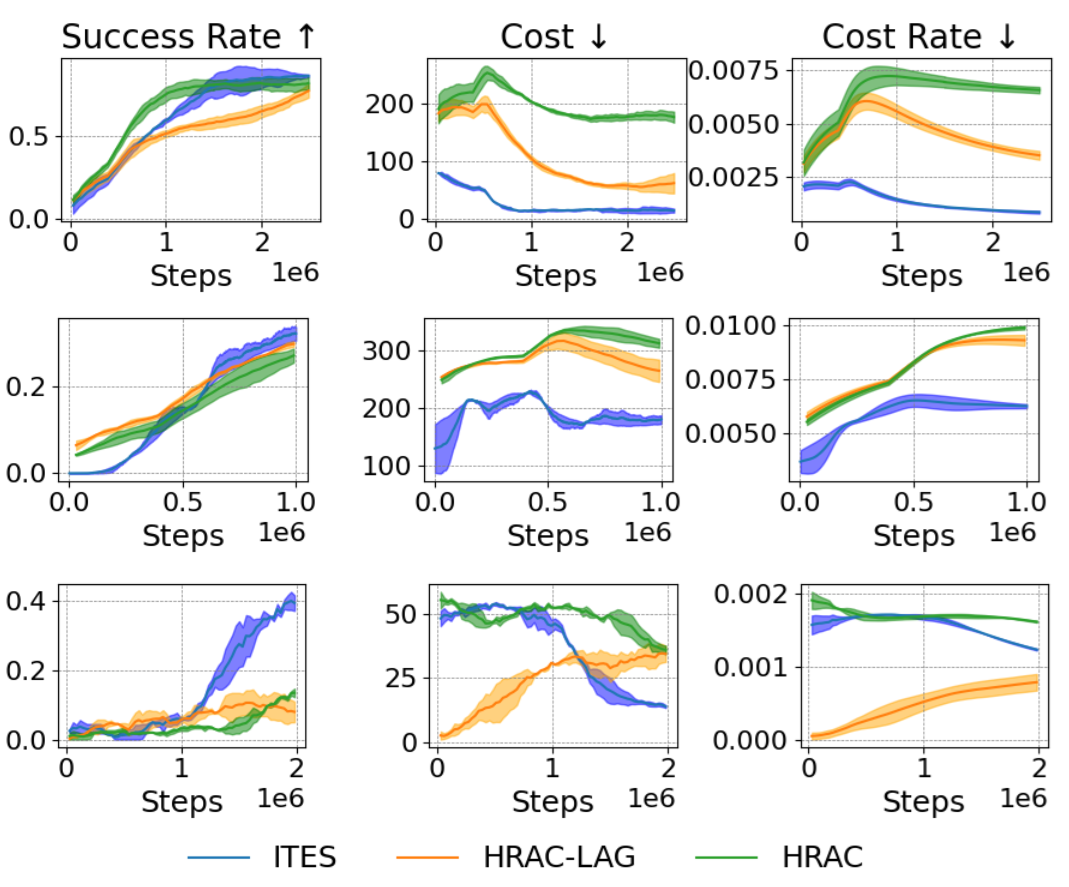
\includegraphics[width=0.88\linewidth]{long_horizon_plots_baselines.png}
    \caption{\textbf{Сравнение с базовыми методами на бенчмарках SafeAntMaze и SafePusher}. Сравнение предложенного метода ITES с безопасным иерархическим методом HRAC-LAG и небезопасным методом HRAC. \textbf{Первая строка}: среда SafeAntMazeCshape. \textbf{Вторая строка}: среда SafeAntMazeWshape. \textbf{Третья строка}: среда SafePusher. Каждый запуск проводился по 5 случайным инициализациям. Заштрихованная область соответствует стандартному отклонению.}
    \label{fig:baselines_compartion_safe_ant_maze}
\end{figure}

\subsection{Сравнение ITES с базовыми методами на задачах с коротким горизонтом}
\label{subsec:ites_rq3}

На рис.~\ref{fig:baselines_compartion_safety_gym_point} показано сравнение с иерархическими стратегиями на бенчмарке Safety Gym. В средах PointGoal1 и CarGoal1 предложенный метод превосходит HRAC-LAG по безопасности при сопоставимой доле успешных эпизодов.

\begin{figure}[!t]
    \centering
    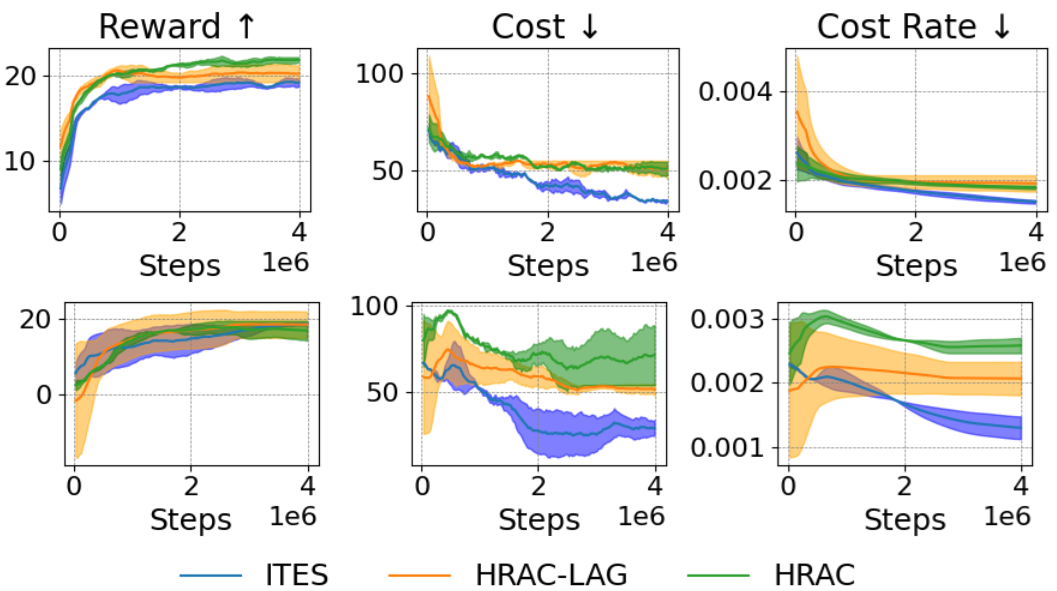
\includegraphics[width=0.88\linewidth]{short_horizon_plots_baselines.png}
    \caption{\textbf{Сравнение с базовыми методами на Safety Gym}. \textbf{Первая строка}: PointGoal1. \textbf{Вторая строка}: CarGoal1. Результаты усреднены по 5 случайным запускам.}
    \label{fig:baselines_compartion_safety_gym_point}
\end{figure}

Табл.~\ref{tab:table_compartion} содержит сравнение итоговых значений одноуровневых методов CUP и FOCOPS с предложенным методом ITES на Safety Gym. В среде CarGoal1, где динамика агента сложнее, а размерность пространства состояний больше, чем в PointGoal1, одноуровневые методы хуже сохраняют высокую эффективность: TD3-Lagrangian достигает только 8.21, а SafeDreamer --- 6.6. Эти методы переходят к консервативному поведению и решают меньше задач. Из-за этого они могут выглядеть более безопасными, например SafeDreamer имеет нулевой штраф, однако такое поведение является неоптимальным в рамках заданной спецификации безопасности, где стратегия считается безопасной, если её штрафы не превышают $40$. В отличие от них, ITES успешно балансирует эффективность и безопасность, достигая более высокой награды: PointGoal1 --- $19.6$, CarGoal1 --- $18.3$, при сохранении штрафов ниже допустимого порога.

\begin{table}[!t]
\caption{\textbf{Итоговые результаты на бенчмарке Safety Gym.} PG1 --- PointGoal1, CG1 --- CarGoal1, PGs --- PointGoal1 sparse. Для каждой среды используется ограничение штрафов $d=40$. Результаты усреднены по 5 случайным запускам.}
\centering
\resizebox{0.70\linewidth}{!}{
\begin{tabular}{p{0.1\linewidth}p{0.15\linewidth}p{0.19\linewidth}p{0.19\linewidth}}
\toprule
Env & Method & Final Reward$\uparrow$ & Final Cost$\downarrow$ \\
\midrule
& ITES & $\textbf{19.6}\pm 0.46$ & $32.83\pm 1.97$ \\
& TD3LAG & $15.75 \pm 0.39$ & $56.22 \pm 0.85$ \\
& FOCOPS & $14.97 \pm 9.01$ & $33.72 \pm 42.24$ \\
PG1 & CUP & $14.42 \pm 6.74$ & $19.02 \pm 20.08$ \\
& PPOLAG & $12.96 \pm 6.95$ & $25.80 \pm 34.99$ \\
& SafeDreamer & $12 \pm 4$ & $10.3 \pm 9.5$ \\
& MBPPOL & --- & --- \\
\midrule
& ITES & $\textbf{18.3}\pm 0.03$ & $21.72 \pm 0.59$ \\
& FOCOPS & $15.23 \pm 10.76$ & $31.66 \pm 93.51$ \\
& PPOLAG & $13.27\pm 9.26$ & $21.72 \pm 32.06$ \\
CG1 & TD3LAG & $8.21 \pm 6.88$ & $53.7 \pm 9.45$ \\
& SafeDreamer & $6.6 \pm 1.2$ & $0$ \\
& CUP & $6.14 \pm 6.97$ & $36.12 \pm 89.56$ \\
& MBPPOL & --- & --- \\
\midrule
& ITES & $\textbf{8.64}\pm 0.38$ & $33.46\pm 1.47$ \\
& FOCOPS & $7.635 \pm 0.2$ & $22.9 \pm 1.5$ \\
& PPOLAG & $6.85 \pm 0.76$ & $32.645 \pm 5.9$ \\
& MBPPOL & $6.15 \pm 0.15$ & $34.1 \pm 3.6$ \\
PGs & CUP & $1.755 \pm 0.95$ & $12.925 \pm 5.3$ \\
& SafeDreamer & $0.5 \pm 0.5$ & $3.22 \pm 2.34$ \\
& TD3LAG & $0.07 \pm 0.01$ & $64.7 \pm 1.91$ \\
\bottomrule
\end{tabular}
}
\label{tab:table_compartion}
\end{table}

Результаты на среде PointGoal sparse, приведённые в табл.~\ref{tab:table_compartion}, показывают, что простые одноуровневые алгоритмы без модели мира не способны научиться решать задачу: CUP достигает значения 1.755, а TD3LAG --- 0.07. Такие низкие значения показывают, что оба подхода не решают задачу эффективно. В случае CUP агент остаётся неподвижным, что приводит к минимальным штрафам, тогда как TD3LAG выполняет жадные действия, но не может научиться решать задачу в условиях разреженного вознаграждения.

В исходной реализации MBPPOL использует истинную информацию о препятствиях вместо данных лидара во время обучения в средах PointGoal1, PointCar1 и PointGoal sparse. Это приводит к некорректному сравнению, поэтому его значения отмечены знаком ``---''. Тем не менее даже в такой постановке данный подход уступает ITES на задачах PointGoal sparse, поскольку испытывает трудности при обучении в условиях разреженного вознаграждения. SafeDreamer в разреженной постановке достигает итоговой награды только 0.5, так как использует модель награды, обученную на несбалансированном наборе данных из-за разреженности вознаграждения. Это приводит к чрезмерно консервативному поведению, поскольку метод не может научиться решать задачи, требующие большего горизонта, чем исходная PointGoal1. Эти результаты показывают, что при сопоставимых условиях безопасности ITES демонстрирует более высокую эффективность по сравнению с базовыми методами, достигая значения 8.64 и сохраняя ограничения безопасности.

\subsection{Абляционное исследование: влияние компонент ITES на безопасность}
\label{subsec:ites_rq4}

\textbf{Сравнение ITES w/o HLS и ITES w/o LLS}. Чтобы проверить, можно ли обеспечить безопасность только на одном уровне иерархии, ITES сравнивался с двумя вариантами: (i) \textbf{ITES w/o LLS}, где отсутствует безопасность на нижнем уровне, а безопасность обеспечивается только на верхнем уровне; (ii) \textbf{ITES w/o HLS}, где отсутствует безопасность на верхнем уровне, а безопасность обеспечивается только на нижнем уровне. Сравнение проводилось на \textbf{SafeAntMazeCshape}. Как показано на рис.~\ref{fig:ablation_compartion} в первой строке, безопасность на верхнем уровне существенно снижает накопленные штрафы и средний штраф за все время обучения, а добавление безопасности на нижнем уровне дополнительно повышает безопасность и снижает разброс. В частности, ITES w/o LLS показывает более высокую дисперсию штрафов, поскольку агент может нарушать ограничения во время движения к безопасной подцели.

\textbf{Сравнение одноуровневого ITES без верхнего уровня и полного ITES}. Результаты обучения ITES и TD3 с воображаемой безопасностью, вычисляемой с помощью модели мира, обозначенного как TD3IMG, представлены на рис.~\ref{fig:ablation_compartion} во второй строке. Хотя метрика штрафов показывает, что ITES значительно безопаснее TD3IMG, это различие возникает из-за того, что TD3IMG может минимизировать безопасность в воображении только на горизонте 10 шагов, а не до конца эпизода. Увеличить этот горизонт невозможно, поскольку при этом модель мира начинает расходиться. В отличие от TD3IMG, ITES генерирует подцели на 10 шагов вперёд, что позволяет стратегии TD3 безопасно достигать этих целей.

\textbf{Влияние верхнеуровневого критика штрафов $Q^h_c$ на безопасность}. Дополнительно исследовалось, как включение верхнеуровневого критика штрафов $Q^h_c$ в целевую функцию верхнеуровневой стратегии влияет на результат. Соответствующее сравнение приведено на рис.~\ref{fig:ablation_compartion} в третьей строке.

\begin{figure}[!t]
    \centering
    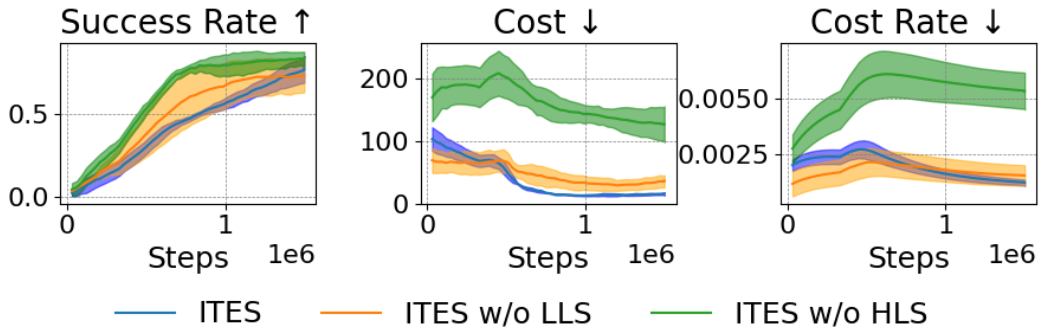
\includegraphics[width=0.88\linewidth]{Ablation_SafeAntMazeCshape_3.png}
    \\
    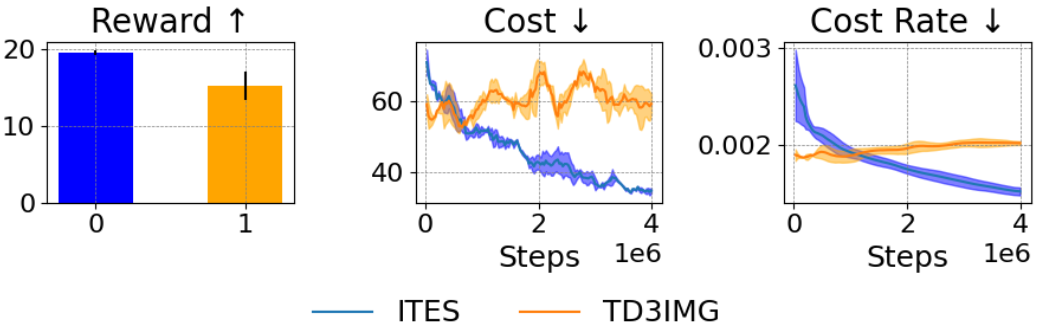
\includegraphics[width=0.88\linewidth]{Ablation_PointGoal1_2.png}
    \\
    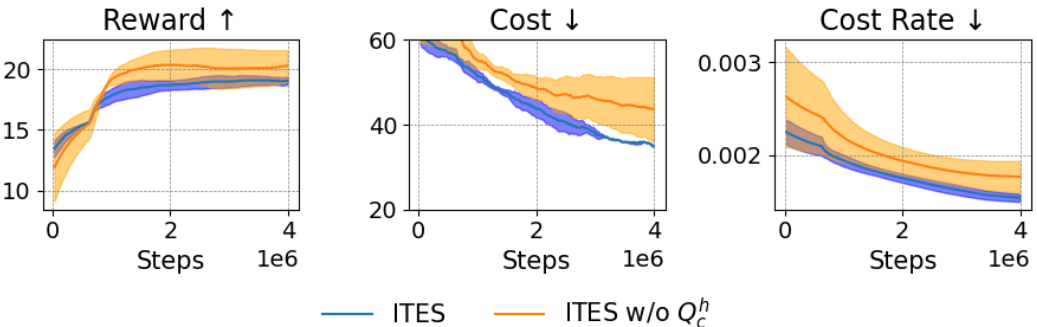
\includegraphics[width=0.88\linewidth]{Ablation_PointGoal1_Q_cost.png}
    \caption{\textbf{Первая строка}: анализ безопасности на нижнем и верхнем уровнях. На рисунке показаны разные варианты ITES: ITES w/o LLS --- ITES без безопасности на нижнем уровне, где безопасность реализуется только на верхнем уровне; ITES w/o HLS --- ITES без безопасности на верхнем уровне, где безопасность реализуется только на нижнем уровне, на SafeAntMazeCshape. \textbf{Вторая строка}: сравнение ITES без верхнеуровневой стратегии и полного ITES на PointGoal1. \textbf{Третья строка}: сравнение ITES и ITES без верхнеуровневого критика штрафов $Q^h_c$ на PointGoal1. Графики получены по 5 случайным запускам.}
    \label{fig:ablation_compartion}
\end{figure}

\section{Выводы по главе}
\label{subsec:ites_conclusion}

В данной главе рассмотрен метод ITES, предназначенный для безопасного обучения в задачах с большим горизонтом. В отличие от одноуровневых методов, ITES использует иерархическую структуру: верхний уровень выбирает промежуточные подцели, а нижний уровень отвечает за их достижение. При этом безопасность учитывается на обоих уровнях. Для выбора подцелей используются модель штрафов и верхнеуровневый критик штрафов, а для низкоуровневой стратегии применяется модель мира, позволяющая проверять воображаемые переходы при движении к подцели.

Эксперименты на SafeAntMaze и SafePusher показывают, что одноуровневые безопасные методы испытывают трудности в задачах большого горизонта. В одних случаях они нарушают ограничение на штраф, в других --- почти не продвигаются к цели и получают низкие штрафы за счёт фактической стагнации. ITES в этих условиях достигает ненулевой доли успешных эпизодов и при этом удерживает штрафы в пределах заданного ограничения в тех постановках, где это требуется спецификацией эксперимента.

На задачах Safety Gym с более коротким горизонтом метод также остаётся конкурентоспособным. В PointGoal1, CarGoal1 и PointGoal sparse ITES сохраняет штрафы ниже допустимого порога и при этом получает более высокое итоговое вознаграждение по сравнению с большинством базовых методов. Это показывает, что иерархическая структура не приводит к ухудшению качества в более простых задачах, где одноуровневая стратегия уже может быть достаточной.

Таким образом, результаты главы показывают, что в задачах большого горизонта важно контролировать не только действия агента, но и промежуточные цели, через которые строится решение.

